\documentclass[12pt,a4paper]{article}
\usepackage[margin=2.5cm]{geometry}
\usepackage{graphicx}
\usepackage{siunitx}
\usepackage{tikz}
\usepackage{pgfplots}
\usepackage{verbatim}
\usepackage{booktabs}
\pgfplotsset{compat=1.18}
\title{Prefabricated Pedestrian Bridge Concept for IYTE Campus}
\author{Structural Concept Study}
\date{\today}
\begin{document}
\maketitle

\section{Project Overview}
The proposed pedestrian bridge is a single span, prefabricated reinforced concrete structure that will cross a seasonal drainage line near the coordinates $(38.31837^{\circ}\,\mathrm{N},\,26.63860^{\circ}\,\mathrm{E})$ within the İzmir Institute of Technology (IYTE) campus. A clear span of \SI{10}{\meter} is sufficient to avoid interference with the existing landscaping while maintaining minimal foundation footprints. The bridge is intended for pedestrian and light service vehicle access (golf carts and maintenance carts with axle loads below \SI{10}{\kilo\newton}). The deck width of \SI{3.0}{\meter} accommodates two-way pedestrian traffic and barrier clearances.

\section{Concept and Structural Form}
The deck consists of two identical precast girders spaced at \SI{1.5}{\meter}, supporting a composite cast-in-place concrete walking slab. Each girder acts as a T-beam with a \SI{1.50}{\meter} wide flange and \SI{0.12}{\meter} slab thickness. The precast web is \SI{0.25}{\meter} wide and \SI{0.90}{\meter} deep, providing sufficient stiffness for the \SI{10}{\meter} span. Prefabrication minimizes on-site construction time and limits work adjacent to the drainage channel. Bridge railings are fixed to embedded plates cast into the slab edge beams.

The bridge bearings are elastomeric pads resting on reinforced concrete seat blocks founded on shallow spread footings. Drainage is directed away from the channel using a \SI{2}{\percent} crossfall toward scuppers located at each abutment.

\section{Design Basis}
Design loads follow TS~498 for pedestrian bridges (uniform pedestrian load of \SI{5}{\kilo\newton\per\square\meter}) and TS~500 for reinforced concrete member design. Material strengths are summarised in Table~\ref{tab:materials}. Partial safety factors of $\gamma_G = 1.4$ for permanent loads and $\gamma_Q = 1.6$ for imposed loads are adopted, consistent with TS~500 ultimate limit state (ULS) combinations.

\begin{table}[h]
\centering
\begin{tabular}{llr}
\toprule
Material & Grade & Design value \\
\midrule
Concrete & C40/50 & $f_{ck}=\SI{40}{\mega\pascal}$, $f_{cd}=\SI{22.7}{\mega\pascal}$ \\
Reinforcing steel & B420C & $f_{yk}=\SI{420}{\mega\pascal}$, $f_{yd}=\SI{365}{\mega\pascal}$ \\
\bottomrule
\end{tabular}
\caption{Material strengths used in the design.}
\label{tab:materials}
\end{table}

\section{Loading and Global Effects}
Each girder supports a \SI{1.5}{\meter} tributary width of deck. The Python companion script reports the same values shown in Table~\ref{tab:loads}, enabling quick sensitivity studies during review.

\begin{table}[h]
\centering
\begin{tabular}{lcc}
\toprule
Load component & Unfactored load (kN/m) & Description \\
\midrule
Precast girder self-weight & 5.63 & $25\,\mathrm{kN/m^3}\times0.25\times0.90$ \\
Composite deck slab & 4.50 & $25\,\mathrm{kN/m^3}\times1.5\times0.12$ \\
Wearing surface and utilities & 1.50 & Allowance for tiles, conduits \\
Steel railing line load & 1.00 & TS~498 minimum \\
Pedestrian live load & 7.50 & $5.0\,\mathrm{kN/m^2}\times1.5$ \\
\midrule
Total permanent load $G$ & 12.63 & Sum of self-weight items \\
Imposed load $Q$ & 7.50 & Pedestrian live load \\
\bottomrule
\end{tabular}
\caption{Characteristic line loads per girder.}
\label{tab:loads}
\end{table}

The governing ultimate line load is $w_{Ed} = 1.4G + 1.6Q = \SI{29.67}{\kilo\newton\per\meter}$. The maximum bending moment and support shear for the simply supported \SI{10}{\meter} span are
\begin{align*}
M_{Ed} &= \frac{w_{Ed}L^2}{8} = \SI{371}{\kilo\newton\meter}, \\
V_{Ed} &= \frac{w_{Ed}L}{2} = \SI{148}{\kilo\newton}.
\end{align*}

Serviceability checks use the unfactored load $w_{ser} = G + Q = \SI{20.13}{\kilo\newton\per\meter}$, matching the "service" line load reported by the Python script.

\section{Section Design}
The chosen reinforcement arrangement comprises four \SI{20}{\milli\meter} diameter B420C bars (area $A_s = \SI{1257}{\square\milli\meter}$) placed with \SI{45}{\milli\meter} cover. The design software (Appendix~\ref{app:python}) evaluates the required steel area ($A_{s,req} = \SI{1071}{\square\milli\meter}$) and the resulting design moment capacity $M_{Rd} = \SI{435}{\kilo\newton\meter} > M_{Ed}$. The neutral axis remains inside the flange ($x = \SI{19}{\milli\meter}$), confirming singly reinforced behaviour.

The web width of \SI{250}{\milli\meter} provides sufficient shear capacity when supplemented with two-legged \SI{10}{\milli\meter} closed stirrups at \SI{200}{\milli\meter} spacing. Concrete shear resistance $V_{Rd,c} = \SI{115}{\kilo\newton}$ and the provided transverse reinforcement adds $V_{Rd,s} = \SI{247}{\kilo\newton}$, comfortably exceeding $V_{Ed}$. The maximum allowable shear resistance $V_{Rd,max} = \SI{2455}{\kilo\newton}$ is not governing.

\section{Serviceability}
With an elastic modulus $E_{cm}=\SI{34}{\giga\pascal}$ (TS~500 for C40/50) and the gross second moment of area $I_g = \SI{4.14\times10^{-2}}{\meter^4}$, the midspan deflection under service loading is
\[
\delta_{max} = \frac{5w_{ser}L^4}{384E_{cm}I_g} = \SI{1.9}{\milli\meter} < \frac{L}{500} = \SI{20}{\milli\meter}.
\]
Crack width control is satisfied by limiting the bar spacing to \SI{150}{\milli\meter} within the flange; the low tensile stress (neutral axis close to the compression face) and the cover thickness meet TS~500 crack control guidance.

\section{Software Cross-Checks}

The open-source tooling cited in the project brief is incorporated through helper scripts. Table~\ref{tab:software} summarises the available verifications and their installation commands.

\begin{table}[h]
\centering
\begin{tabular}{lll}
\toprule
Library & Helper file & Usage notes \\
\midrule
\texttt{concreteproperties} & \texttt{concreteproperties\_check.py} & Computes $M_{Rd}$ via non-linear section analysis. \\
\texttt{rcdesign} & \texttt{rcdesign\_check.py} & Reproduces the limit-state report in IS~456 notation. \\
\bottomrule
\end{tabular}
\caption{Optional software verification resources (see \texttt{docs/pedestrian\_bridge}).}
\label{tab:software}
\end{table}

The main calculation script detects whether the optional packages are available and records the outcome in its console report so that reviewers can confirm consistency with these external tools.

\section{Constructability and Detailing}
Each girder weighs approximately \SI{28}{\kilo\newton} and can be transported using campus maintenance equipment. Lifting anchors are cast into the web at third points. After erection, a \SI{120}{\milli\meter} thick topping slab is poured to create the walking surface and integrate the two precast units. Stainless steel drainage scuppers and guardrail posts are embedded during casting. Elastomeric bearings (\SI{350\times350\times50}{\milli\meter}) isolate girder rotations at the abutments.

\section{Drawings}
Figures~\ref{fig:section} and~\ref{fig:3d} illustrate the cross-section and an axonometric view generated directly from the design parameters.

\begin{figure}[h]
\centering
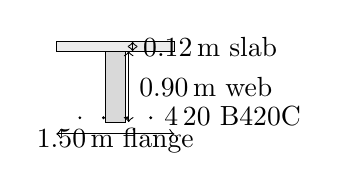
\begin{tikzpicture}[scale=1]
    % parameters in mm scaled to cm (1cm=100mm)
    \def\bf{1.5}
    \def\tf{0.12}
    \def\bw{0.25}
    \def\hw{0.9}
    \def\cover{0.045}
    \def\bard{0.02}
    % draw flange
    \draw[fill=gray!15] (-0.75,\hw) rectangle (0.75,\hw+\tf);
    % draw web
    \draw[fill=gray!30] (-0.125,0) rectangle (0.125,\hw);
    % dimension lines
    \draw[<->] (-0.75, -0.15) -- (0.75,-0.15);
    \node at (0,-0.23) {\SI{1.50}{\meter} flange};
    \draw[<->] (0.17,0) -- (0.17,\hw);
    \node[anchor=west] at (0.18,\hw/2) {\SI{0.90}{\meter} web};
    \draw[<->] (0.22,\hw) -- (0.22,\hw+\tf);
    \node[anchor=west] at (0.23,\hw+\tf/2) {\SI{0.12}{\meter} slab};
    % reinforcement bars
    \foreach \x in {-0.45,-0.15,0.15,0.45} {
        \draw[fill=black] (\x,\cover+\bard/2) circle (0.01);
    }
    \node[anchor=west] at (0.5,0.08) {$4\,\varnothing20$ B420C};
\end{tikzpicture}
\caption{T-beam cross-section per girder (dimensions to scale).}
\label{fig:section}
\end{figure}

\begin{figure}[h]
\centering
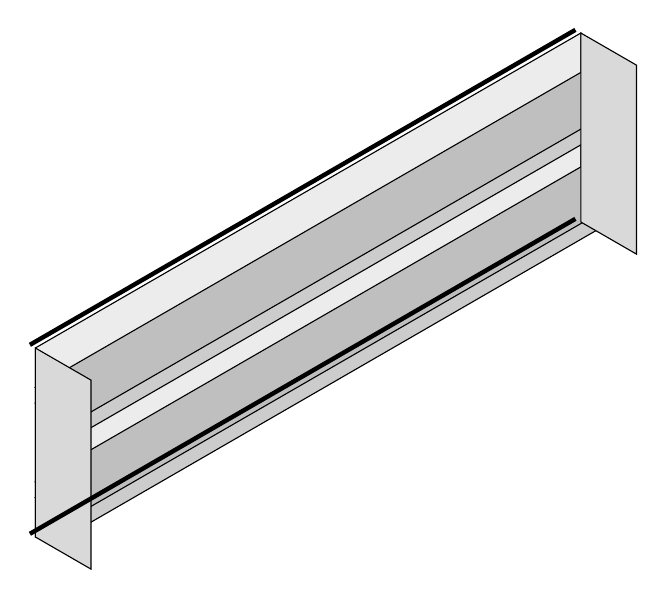
\begin{tikzpicture}[scale=0.8, x={(0.866cm,0.5cm)}, y={(0cm,1cm)}, z={( -0.866cm,0.5cm)}]
    \def\span{10}
    \def\width{3}
    \def\depth{1.02}
    \def\webw{0.25}
    \def\spacing{1.5}
    % deck slab
    \draw[fill=gray!15] (0,0,0) -- (\span,0,0) -- (\span,\width,0) -- (0,\width,0) -- cycle;
    % webs
    \foreach \y in {0.75,2.25} {
        \draw[fill=gray!40] (0,\y-\webw/2,0) -- (\span,\y-\webw/2,0) -- (\span,\y-\webw/2,-\depth+0.12) -- (0,\y-\webw/2,-\depth+0.12) -- cycle;
        \draw[fill=gray!50] (0,\y+\webw/2,0) -- (\span,\y+\webw/2,0) -- (\span,\y+\webw/2,-\depth+0.12) -- (0,\y+\webw/2,-\depth+0.12) -- cycle;
    }
    % girder ends
    \draw[fill=gray!30] (0,0,0) -- (0,\width,0) -- (0,\width,-\depth) -- (0,0,-\depth) -- cycle;
    \draw[fill=gray!30] (\span,0,0) -- (\span,\width,0) -- (\span,\width,-\depth) -- (\span,0,-\depth) -- cycle;
    % simple railing indication
    \draw[ultra thick] (0,0,0.1) -- (\span,0,0.1);
    \draw[ultra thick] (0,\width,0.1) -- (\span,\width,0.1);
\end{tikzpicture}
\caption{Axonometric visualisation of the prefabricated twin-girder system.}
\label{fig:3d}
\end{figure}

\section{Conclusions}
The analysis confirms that the selected prefabricated T-beam concept satisfies TS~500 ultimate and serviceability requirements with reserve capacity for moderate future load increases (e.g., light utility vehicles). The layout integrates seamlessly with the campus landscape and can be executed with minimal site disruption. Detailed reinforcement schedules and bearing layouts can be developed directly from the presented calculations.

\appendix
\section{Calculation Extracts}\label{app:python}
The numerical results in this report are generated by the Python script in Listing~\ref{lst:python}, which follows the procedures outlined by TS~500 for T-beam design.

\begin{figure}[h]
\centering
\begin{minipage}{0.95\linewidth}
\scriptsize
\verbatiminput{../../design/pedestrian_bridge/design.py}
\end{minipage}
\caption{Python script used for design verification.}
\label{lst:python}
\end{figure}

The directory further includes \texttt{concreteproperties\_check.py} and \texttt{rcdesign\_check.py}, which execute the optional software validations listed in Section~\ref{tab:software}.


\end{document}
